
\section{Components Used}
\begin{figure}[H]

\begin{subfigure}{0.5\textwidth}
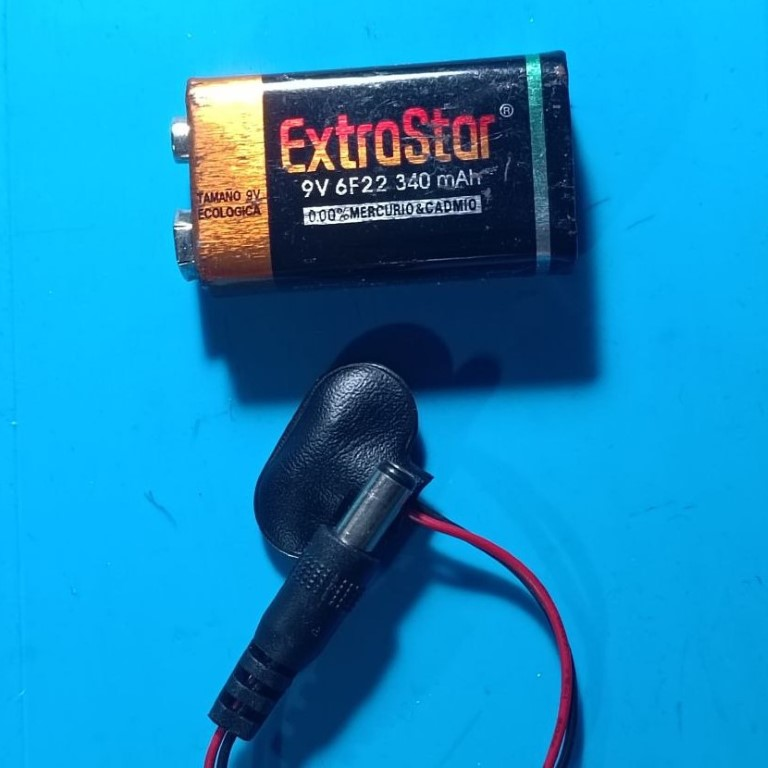
\includegraphics[width=0.9\linewidth, height=6cm]{medias/parts/9v_battery.jpg} 
\caption{Battery 9V}
\label{fig:battery}
\end{subfigure}
\begin{subfigure}{0.5\textwidth}
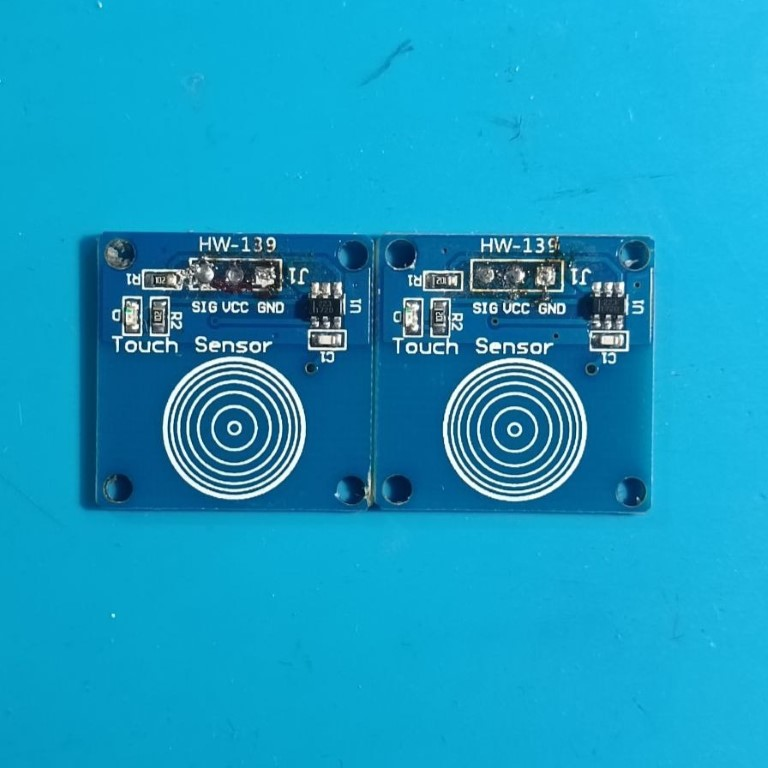
\includegraphics[width=0.9\linewidth, height=6cm]{medias/parts/touch_sensor.jpg}
\caption{Touch Button (HW-139)}
\label{fig:touchbutton}
\end{subfigure}

\begin{subfigure}{0.5\textwidth}
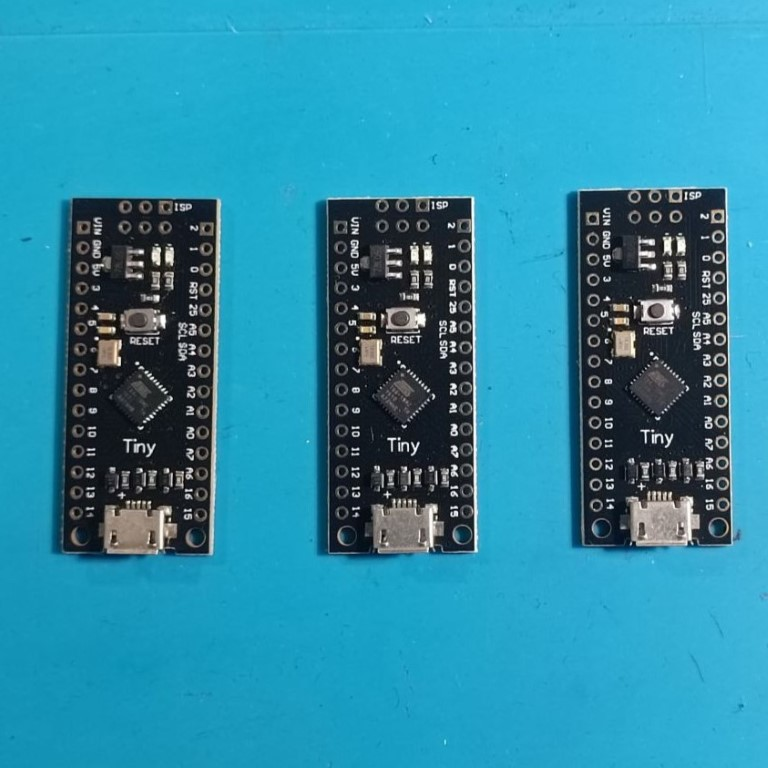
\includegraphics[width=0.9\linewidth, height=6cm]{medias/parts/board.jpg} 
\caption{ATtiny or Arduino Nano}
\label{fig:board}
\end{subfigure}
\begin{subfigure}{0.5\textwidth}
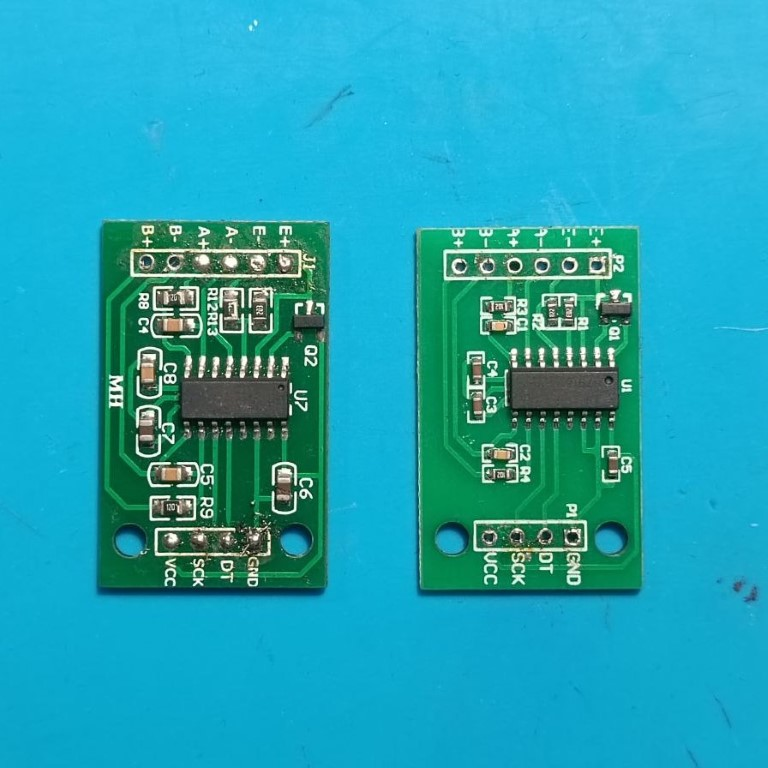
\includegraphics[width=0.9\linewidth, height=6cm]{medias/parts/hx711.jpg}
\caption{HX711}
\label{fig:hx711}
\end{subfigure}
\caption{}
\end{figure}

The \textbf{9V battery} is used as a portable power source for the project.\\
\\
The \textbf{HW-139 touch button} is a component used for touch detection. It can be used as a tare button for resetting the scale.\\\\
The \textbf{ATtiny} or \textbf{Arduino Nano} are some examples of a microcontroller development board used for programming and controlling the scale and its components.  \\ 
\\
The \textbf{HX711} is used to amplify and convert the analog signal from the load cell into a digital one that can be read by the microcontroller.\\
\\


\begin{figure}[H]
\begin{subfigure}{0.5\textwidth}
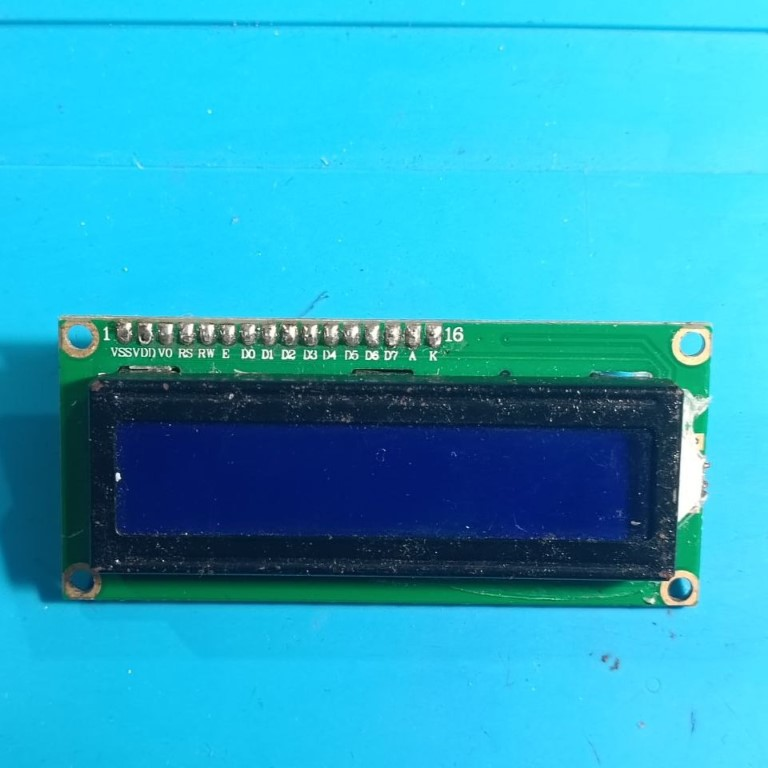
\includegraphics[width=0.9\linewidth, height=6cm]{medias/parts/i2c_Screen.jpg} 
\caption{I2C Screen}
\label{fig:i2c}
\end{subfigure}
\begin{subfigure}{0.5\textwidth}
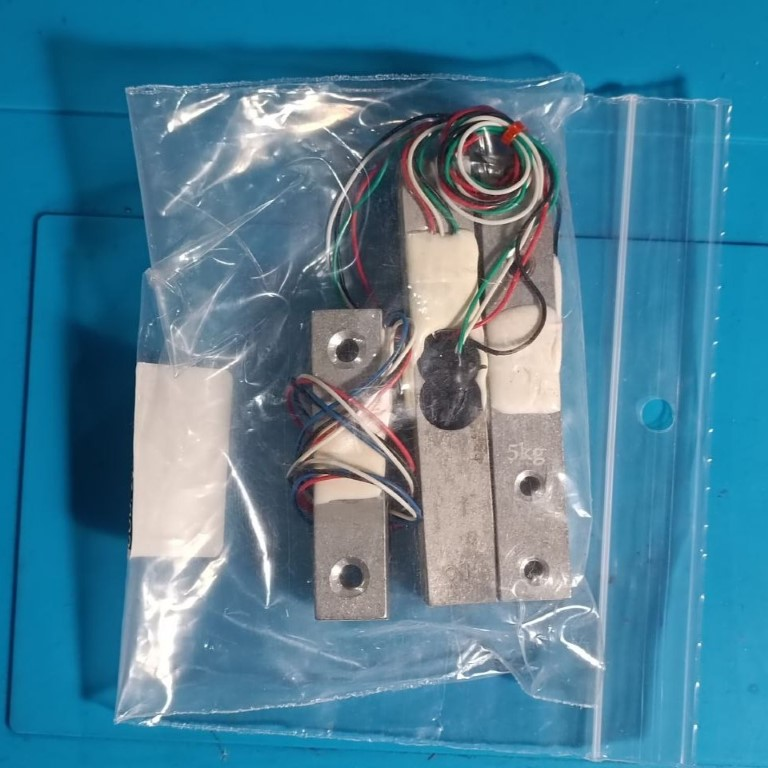
\includegraphics[width=0.9\linewidth, height=6cm]{medias/parts/load_cell.jpg}
\caption{Loadcell}
\label{fig:loadcell}
\end{subfigure}

\begin{subfigure}{0.5\textwidth}
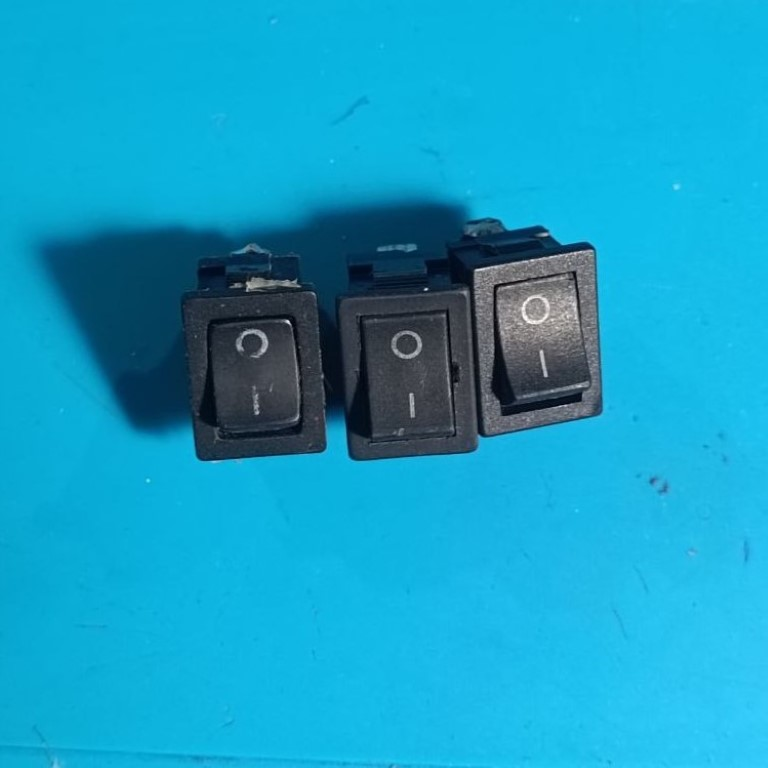
\includegraphics[width=0.9\linewidth, height=6cm]{medias/parts/on_off_switch.jpg} 
\caption{ON-OFF Switch}
\label{fig:switch}
\end{subfigure}
\begin{subfigure}{0.5\textwidth}
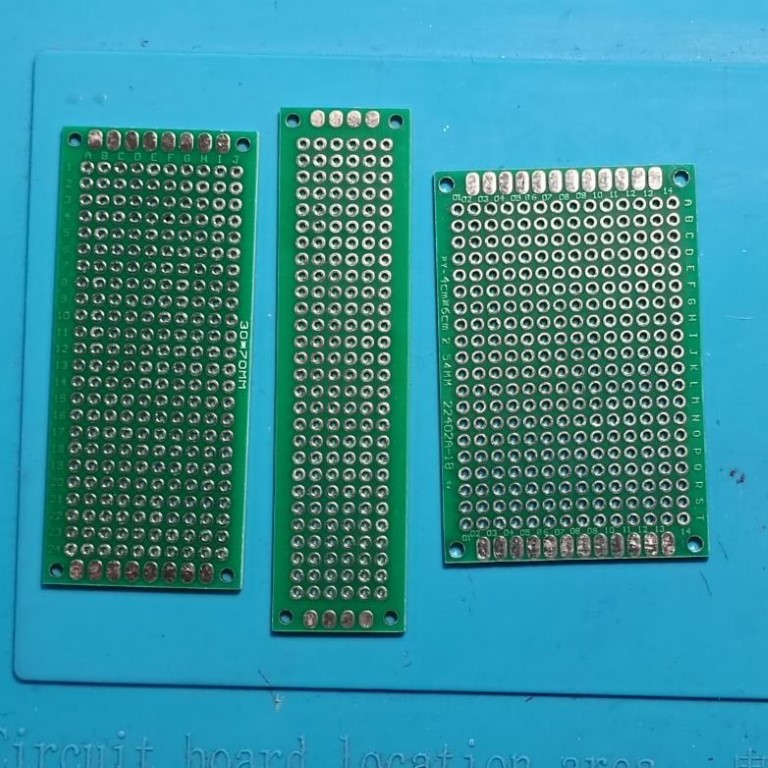
\includegraphics[width=0.9\linewidth, height=6cm]{medias/parts/pcb_board.jpg}
\caption{PCB Board}
\label{fig:pcb}
\end{subfigure}
\caption{}
\end{figure}

\noindent
The \textbf{I2C 16x2 LCD display} is used to show information such as the measured weight or other relevant details. \\
\\
The \textbf{5KG load cell} is a weight sensor used to measure the weight of objects placed on the plate.\\
\\
The \textbf{HX711} is used to amplify and convert the analog signal from the load cell into a digital one that can be read by the microcontroller.\\
\\
The \textbf{PCB} (Printed Circuit Board) is used to connect and organize the electronic components in the project.\\



\begin{figure}[H]
\centering

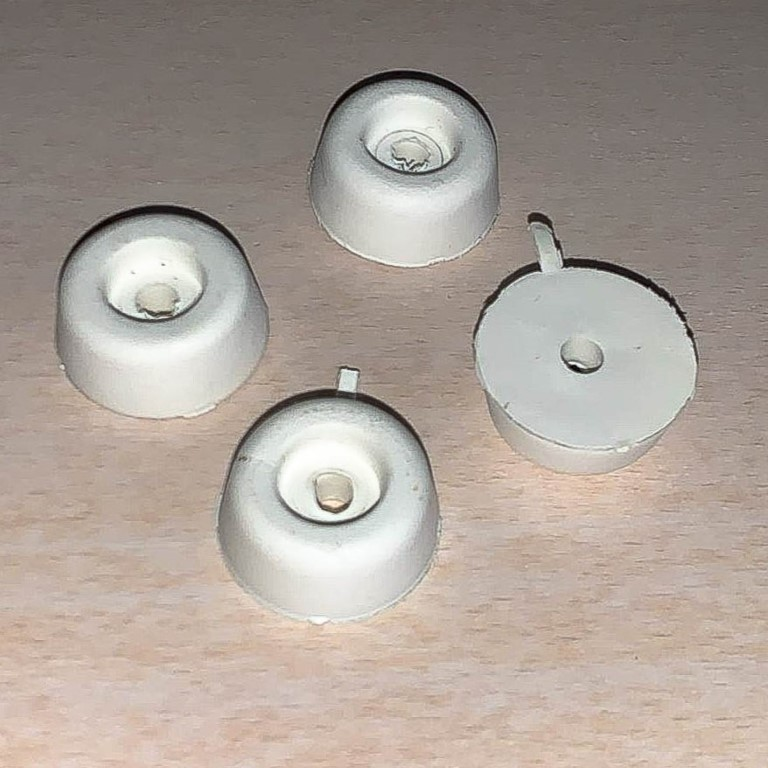
\includegraphics[width=0.5\linewidth, height=6cm]{medias/parts/rubber_support.jpg} 
\caption{Rubber supports}
\label{fig:support}

\end{figure}



\noindent 
\textbf{Rubber supports} needed to avoid sliding and suport the structure of the scale.\\





